\chapter{Application to compact finite difference evaluation}

\section{Introduction}

Here, we discuss the application of the
tridiagonal solver developed in the previous section
to the evaluation of compact finite differences---which
are used widely in the direct numerical simulation
of fluid flows.
%
\begin{figure}
\begin{center}
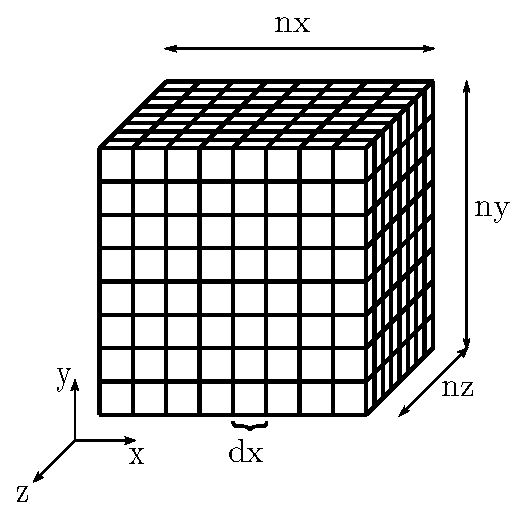
\includegraphics[height=150pt]{img/computational-domain.eps}
\caption{Computational domain in 3-D.}
\label{fig:computational-domain}
\end{center}
\end{figure}
%
In typical DNS applications,
the computational domain considered
is a 3-dimensional,
regular, Cartesian grid with
$nx$, $ny$ and $nz$ grid points and grid spacing of
$dx$, $dy$ and $dz$ in the
respective coordinate directions
(Fig. \ref{fig:computational-domain}).
Structured grids such as these
are widely used because they lend themselves naturally
to finite-difference methods.
To resolve all the spatial features of the flow,
the grid spacing is kept very small.
Consequently,
to simulate flows of practical sizes,
the number of grid points must be very large.
Because of the high computational cost
and memory requirements associated with
the large number of grid points
parallelism becomes mandatory.
We have spoken so far of GPUs as massively parallel systems.
However, each GPU has a very limited amount of global memory:
current NVIDIA Tesla K20 GPUs have about 4 Gigabytes.
Thus, to accommodate the
larger problem sizes in DNS,
the use of \emph{multiple} GPUs is necessary,
which introduces a second level of parallelism.
In the next section,
we describe strategies to distribute
the problem domain among the GPUs
in such dual-level parallel systems.

\section{Compact finite difference evaluation on parallel GPU systems}

The computation of derivatives using
compact finite differences involves two primary steps:

\begin{enumerate}
\item The evaluation of the right hand sides
    of Eq. (\ref{eqn:general-compact})
    at each grid point.
\item The solution of the tridiagonal system
    [Eq. (\ref{eqn:general-compact})]
    for each line of grid points.
\end{enumerate}

Both of these operations are amenable to parallel operations.
The right hand side calculation is a pointwise
\emph{stencil} operation, i.e.,
at every point in the domain,
the value of the right hand side
is computed as a combination of function values
at that point and its neighbouring points.
The stencil operations at individual points
are independent,
making the overall calculation highly parallelizable.
The solution of the tridiagonal systems
is of course parallelizable,
as has been discussed in previous sections.

Without loss of generality,
we consider the parallelization of
compact finite difference evaluations for 2-dimensional problems.
We assume that the derivative is being calulated
for the coordinate direction along which
elements are stored contiguously in memory, i.e.,
the ``fastest'' coordinate direction.

\subsection{Single GPU}

\begin{figure}
\begin{center}
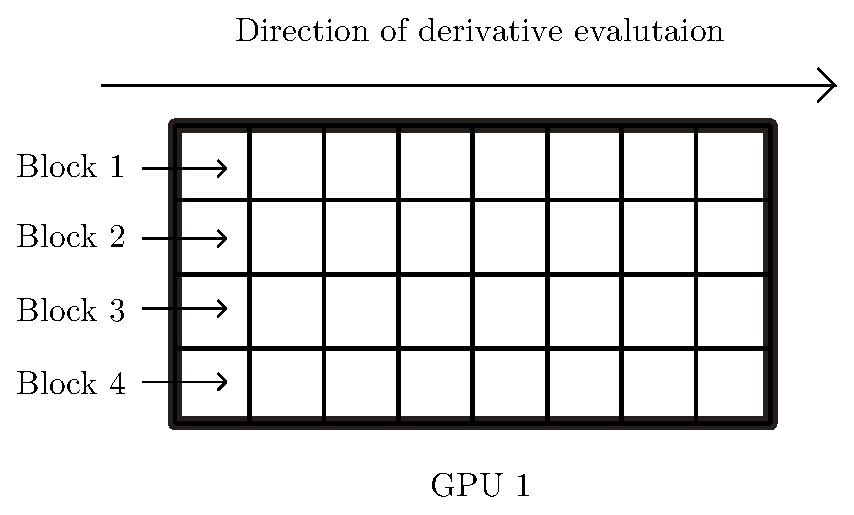
\includegraphics[height=150pt]{img/compact-single-gpu.eps}
\caption{Compact finite differences - single GPU}
\label{fig:compact-single-gpu}
\end{center}
\end{figure}

For a single GPU \ref{fig:compact-single-gpu},
when calculating the right hand sides,
each point in the grid is mapped to a single thread,
and each thread applies the required stencil operation
to compute the right hand side at that point.
We note that threads near the left and right boundaries
apply a different stencil from the interior threads.
The implementation of GPU kernels for
stencil operations such as these is a topic of wide study.
The most important considerations were brought out
in the paper by Micikevicius et al. ~\cite{micikevicius20093d}.
For solving the tridiagonal systems,
each thread block of the GPU is mapped to a
different \emph{grid line}
aligned along the
direction the derivatives are being calculated.
The right hand sides are stored
contiguously along these grid lines
(as in Fig. \ref{fig:block-mapping}),
and the modified cyclic reduction algorithm developed
can be used to solve for the derivatives.

\subsection{Multiple GPUs on a single node}

\begin{figure}
\begin{center}
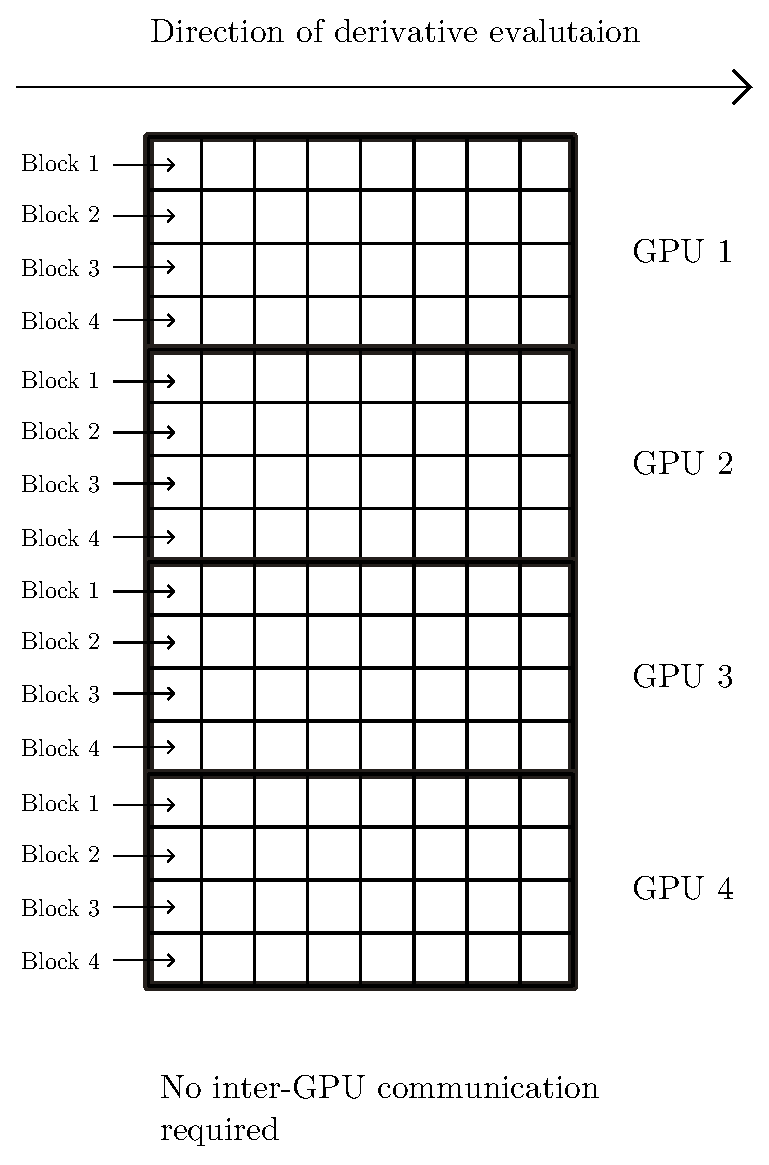
\includegraphics[width=250pt]{img/compact-shared-gpu.eps}
\caption{Compact finite differences - multiple GPUs
    on same node}
\label{fig:compact-shared-gpu}
\end{center}
\end{figure}

Here, we consider the case of multiple GPUs
on a single shared memory node, i.e.,
multiple GPUs attached to the same PCI-e bus.
In this case, every GPU is visible to the host,
and the GPUs read from and write into
the same host memory space.
The domain is divided into a number of
into ``subdomains'',
as shown in \ref{fig:compact-shared-gpu}.
The domain decomposition is done such that
only a single subdomain is used along the
coordinate direction of the derivatives.
This is the method presented by
Sakharnykh et al. ~\cite{sakharnykhADIconf},
and it has the advantage that
no coordination between GPUs is required:
each GPU is assigned an independent
set of grid lines to solve.

\subsection{Distributed GPUs - restricted in one direction}

\begin{figure}
\begin{center}
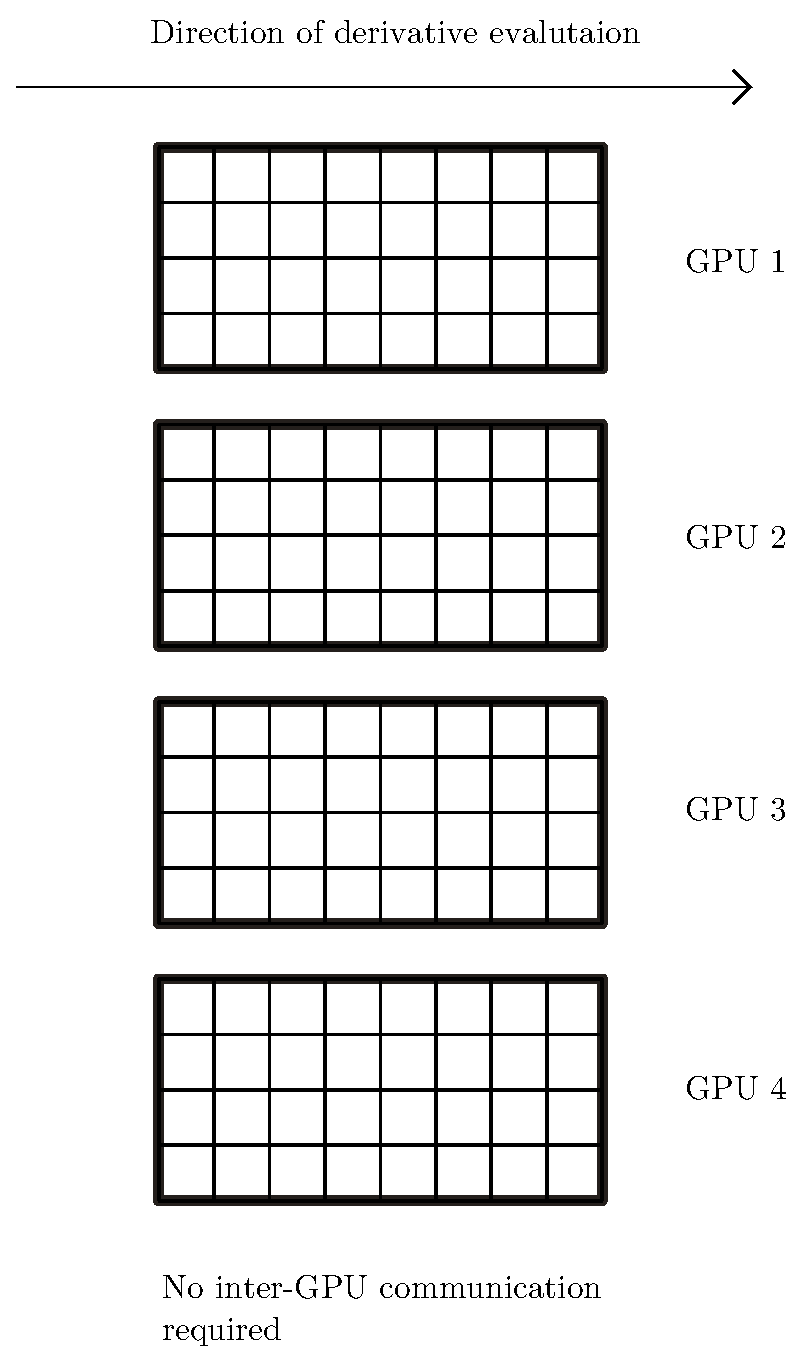
\includegraphics[width=200pt]{img/compact-distributed-restricted.eps}
\caption{Compact finite differences - distributed GPUs and
    restricted in one direction}
\label{fig:compact-distributed-restricted}
\end{center}
\end{figure}

For larger problems,
a distributed system may be required.
Here, the simplest strategy is to use a domain decomposition
as shown in \ref{fig:compact-distributed-restricted}.
Here again, 
no inter-GPU communication is required.
By restricting the distribution along one coordinate direction,
the ease of solution of the tridiagonal systems is maintained.

\subsection{Distributed GPUs in all directions}

\begin{figure}
\begin{center}
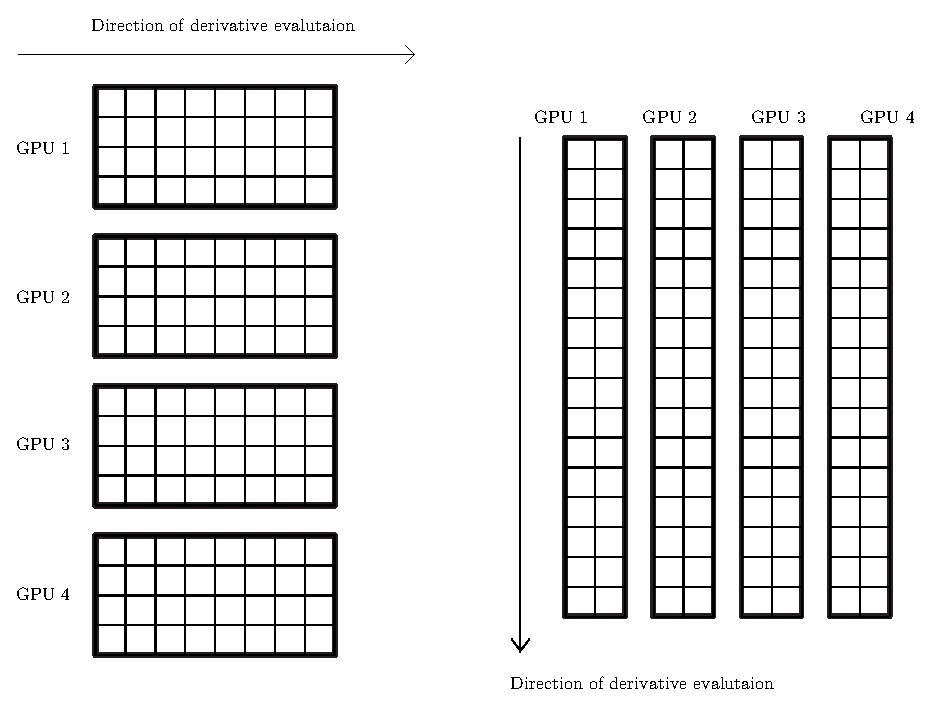
\includegraphics[height=250pt]{img/compact-restricted-transpose.eps}
\caption{Compact finite difference evaluation in both coordinate directions}
\label{fig:compact-restricted-transpose}
\end{center}
\end{figure}

The above domain decomposition strategies are convenient,
but can be impractical for some cases.
For instance,
let us consider the evaluation of derivatives
in the other coordinate direction
(Fig. \ref{fig:compact-restricted-transpose}).
Because the grid lines aligned along this direction
must reside on the same GPU,
it follows that:
%
\begin{enumerate}
\item A \emph{global} transposition or rearrangement
    of the data is required,
    such that each GPU now contains data for
    grid lines aligned in the direction orthogonal
    to the previous direction.
    For distributed systems,
    this transposition can be an extremely expensive process.

\item For domains that are much longer along one coordinate
    direction compared to the other(s),
    the subdomains may become impractically \emph{slender}.
\end{enumerate}
%
Such decomposition strategies are therefore, generally applicable
when compact finite difference schemes are used only
in a single direction.
For the other coordinate directions,
explicit finite difference schemes may be used,
which have the disadvantages discussed earlier.
To accommodate compact finite difference schemes in all the coordinate
directions,
the domain decomposition generally must be performed in all directions,
as shown in Fig. \ref{fig:compact-distributed-all}.
In this strategy,
the grid lines in all coordinate directions
are interrupted by the subdomain boundaries.
Thus,
inter-GPU communication is required.
For the right hand sides evaluation,
each GPU must communicate information at the subdomain boundaries
with neighbouring GPUs.
For example, in Fig. \ref{fig:compact-distributed-all},
the right-most grid points in the subdomain of
GPU 2 require data from the
left-most grid points in the subdomain of
GPU 6 when evaluating derivatives in the horizontal direction.
Similarly,
the left-most grid points in the subdomain of
GPU 6 require data from the
right-most grid points in the subdomain of
GPU 2.
Thus, a ``swapping'' of the boundary information
is required at each of the subdomain boundaries.

The solution of the distributed tridiagonal systems
involves much more complexity,
and is discussed in detail in the next section.

\begin{figure}
\begin{center}
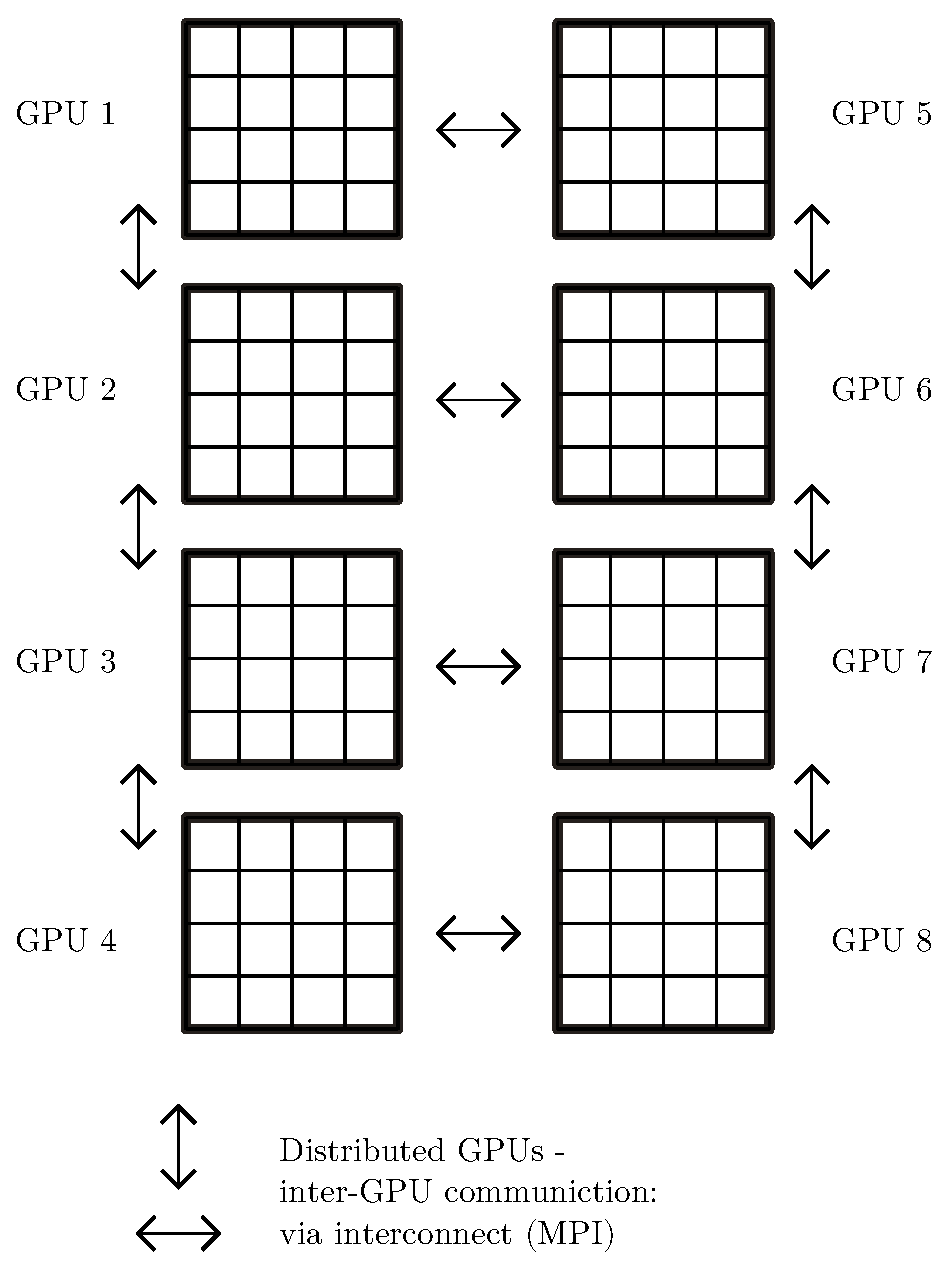
\includegraphics[width=200pt]{img/compact-distributed-all.eps}
\caption{Compact finite differences - distributed GPUs in all
    directions}
\label{fig:compact-distributed-all}
\end{center}
\end{figure}

\section{Distributed tridiagonal solver}

\subsection{General algorithm}
\label{subsec:distributed-tridiagonal-algorithm}

We use the algorithm
proposed by Mattor et al. \cite{mattor1995algorithm}
for solving the distributed tridiagonal systems.
For a general tridiagonal system $A\bm{x}=\bm{r}$,
the algorithm begins by partitioning
the matrix and right-hand side among the $P$ processes.
Each process $p$ is then associated with the
following $\emph{subsystems}$

\begin{align}
    & A^p\bm{u}^p = \bm{r_u}^p & \label{eqn:secondary-system-1} \\ 
    & A^p\bm{l}^p = \bm{r_l}^p & \label{eqn:secondary-system-2} \\
    & A^p\bm{x_r}^p = \bm{r}^p & \label{eqn:primary-system} 
\end{align}
%
expanded as:

\begin{align}
& \begin{bmatrix}
b_1^p & c_1^p \\
a_2^p & b_2^p & c_2^p \\
      & a_3^p & b_3^p & c_3^p \\
      &       & a_4^p & b_4^p & c_4^p \\
      &       &       &       &  \ddots & c_{m-1}^p\\
      &       &       &       &     a_{m}^p  & b_{m}^p
\end{bmatrix}
\begin{bmatrix}
x_{r,1}^p \\
x_{r,2}^p \\
x_{r,3}^p \\
x_{r,4}^p \\
\vdots \\
x_{r,m}^p
\end{bmatrix}
=
\begin{bmatrix}
r_1^p \\
r_2^p \\
r_3^p \\
r_4^p \\
\vdots \\
r_m^p
\end{bmatrix} & \label{eqn:primary-system-expanded} \\
\end{align}

\begin{align}
& \begin{bmatrix}
b_1^p & c_1^p \\
a_2^p & b_2^p & c_2^p \\
      & a_3^p & b_3^p & c_3^p \\
      &       & a_4^p & b_4^p & c_4^p \\
      &       &       &       &  \ddots & c_{m-1}^p\\
      &       &       &       &     a_{m}^p  & b_{m}^p
\end{bmatrix}
\begin{bmatrix}
u_1^p \\
u_2^p \\
u_3^p \\
u_4^p \\
\vdots \\
u_m^p
\end{bmatrix}
=
\begin{bmatrix}
-a_1^p \\
0 \\
0 \\
0 \\
\vdots \\
0
\end{bmatrix} & \label{eqn:secondary-system-1-expanded} \\
\end{align}
%
\begin{align}
& \begin{bmatrix}
b_1^p & c_1^p \\
a_2^p & b_2^p & c_2^p \\
      & a_3^p & b_3^p & c_3^p \\
      &       & a_4^p & b_4^p & c_4^p \\
      &       &       &       &  \ddots & c_{m-1}^p\\
      &       &       &       &     a_{m}^p  & b_{m}^p
\end{bmatrix}
\begin{bmatrix}
l_1^p \\
l_2^p \\
l_3^p \\
l_4^p \\
\vdots \\
l_m^p
\end{bmatrix}
=
\begin{bmatrix}
0 \\
0 \\
0 \\
0 \\
\vdots \\
-c_m^p
\end{bmatrix} & \label{eqn:secondary-system-2-expanded}
\end{align}
%
We refer to the subsystem in Eq. (\ref{eqn:primary-system-expanded})
the ``primary'' system, and the subsystems in
Eqs. (\ref{eqn:secondary-system-1-expanded}) and
(\ref{eqn:secondary-system-2-expanded})
the ``secondary'' systems.
Additionally, the following ``reduced'' system is solved:

\begin{align} \label{eqn:reduced-system}
&
\begin{bmatrix}
l^1_m & -1 \\
-1    & u^2_1 & l^2_1 \\
      & u^2_m & l^2_m & -1 \\
      &       & -1    & u^3_1 & l^3_1 \\
      &       &       & u^3_m & l^3_m  & -1 \\
      &       &       &       & \ddots & \ddots & \ddots \\
      &       &       &       &        & -1     & u^P_1
\end{bmatrix}
\begin{bmatrix}
\beta^1 \\
\alpha^2 \\
\beta^2 \\
\alpha^3 \\
\beta^3 \\
\vdots \\
\alpha^P
\end{bmatrix}
=
\begin{bmatrix}
x_{r,m}^1 \\
x_{r,1}^2 \\
x_{r,m}^2 \\
x_{r,1}^3 \\
x_{r,m}^3 \\
\vdots \\
x_{r,1}^P \\
\end{bmatrix}
&
\end{align}
The local part of the solution
is obtained as a linear combination of
the solutions to the primary and secondary systems:

\begin{equation}
    \bm{x}^p = \bm{x}_r^p + \
        \alpha^p \bm{u}^p + \beta^p \bm{l}^p
    \label{eqn:sum-of-systems}
\end{equation}
%
where $\alpha^p$ and $\beta^p$ are obtained
from the solution of the reduced system.

\subsection{Specialization for compact finite difference
    evaluations}

The algorithm described in
Sec. \ref{subsec:distributed-tridiagonal-algorithm}
is applicable to a single tridiagonal system distributed
across several processors.
When solving a distributed tridiagonal system
for several distributed grid lines,
we note that
the secondary systems
[Eq. (\ref{eqn:secondary-system-1-expanded}) and
 Eq. (\ref{eqn:secondary-system-2-expanded})]
are dependent only on $\bm{a}$, $\bm{b}$ and $\bm{c}$,
the tridiagonal coefficients of the global tridiagonal system.
These are the same for all local grid lines,
so they are solved for a single local grid line in each subdomain.
Only the system in Eq. (\ref{eqn:primary-system-expanded})
is solved for all the grid lines in a subdomain.
For a single tridiagonal system,
the reduced system requires \emph{global} communication
of the values $\{u^p_1, u^p_m\, l^p_1, l^p_m\, x^p_{r,1} x^p_{r,m}\}$
from each process $p$.
When solving for several grid lines,
the left hand side may be assembled for a single grid line.
The right hand sides, however, must be assembled for every grid line,
and the system is solved for each right hand side.

\section{GPU implementation}

Our algorithm is outlined in \ref{fig:compact-algorithm},
and is described for the case of evaluating derivatives
in the direction along which successive
function values in a subdomain are stored contiguously in memory,
i.e., the ``fastest'' coordinate direction.
Each step of the algorithm must be implemented on the GPU
to avoid data transfer to and from the CPU,
which is prohibitively expensive for large problems.
Thus, we have several kernels to implement the algorithm.
For communication of data between processes,
we use the Message Passing Interface (MPI),
and leverage the NVIDIA GPUDirect Technology
for GPU-GPU communication.
MPI is interfaced via the mpi4py \cite{dalcin2005mpi}
Python library.
The purpose of each CUDA kernel and MPI call used
is described in Table \ref{table:compact-algorithm}.

\begin{figure}
\begin{center}
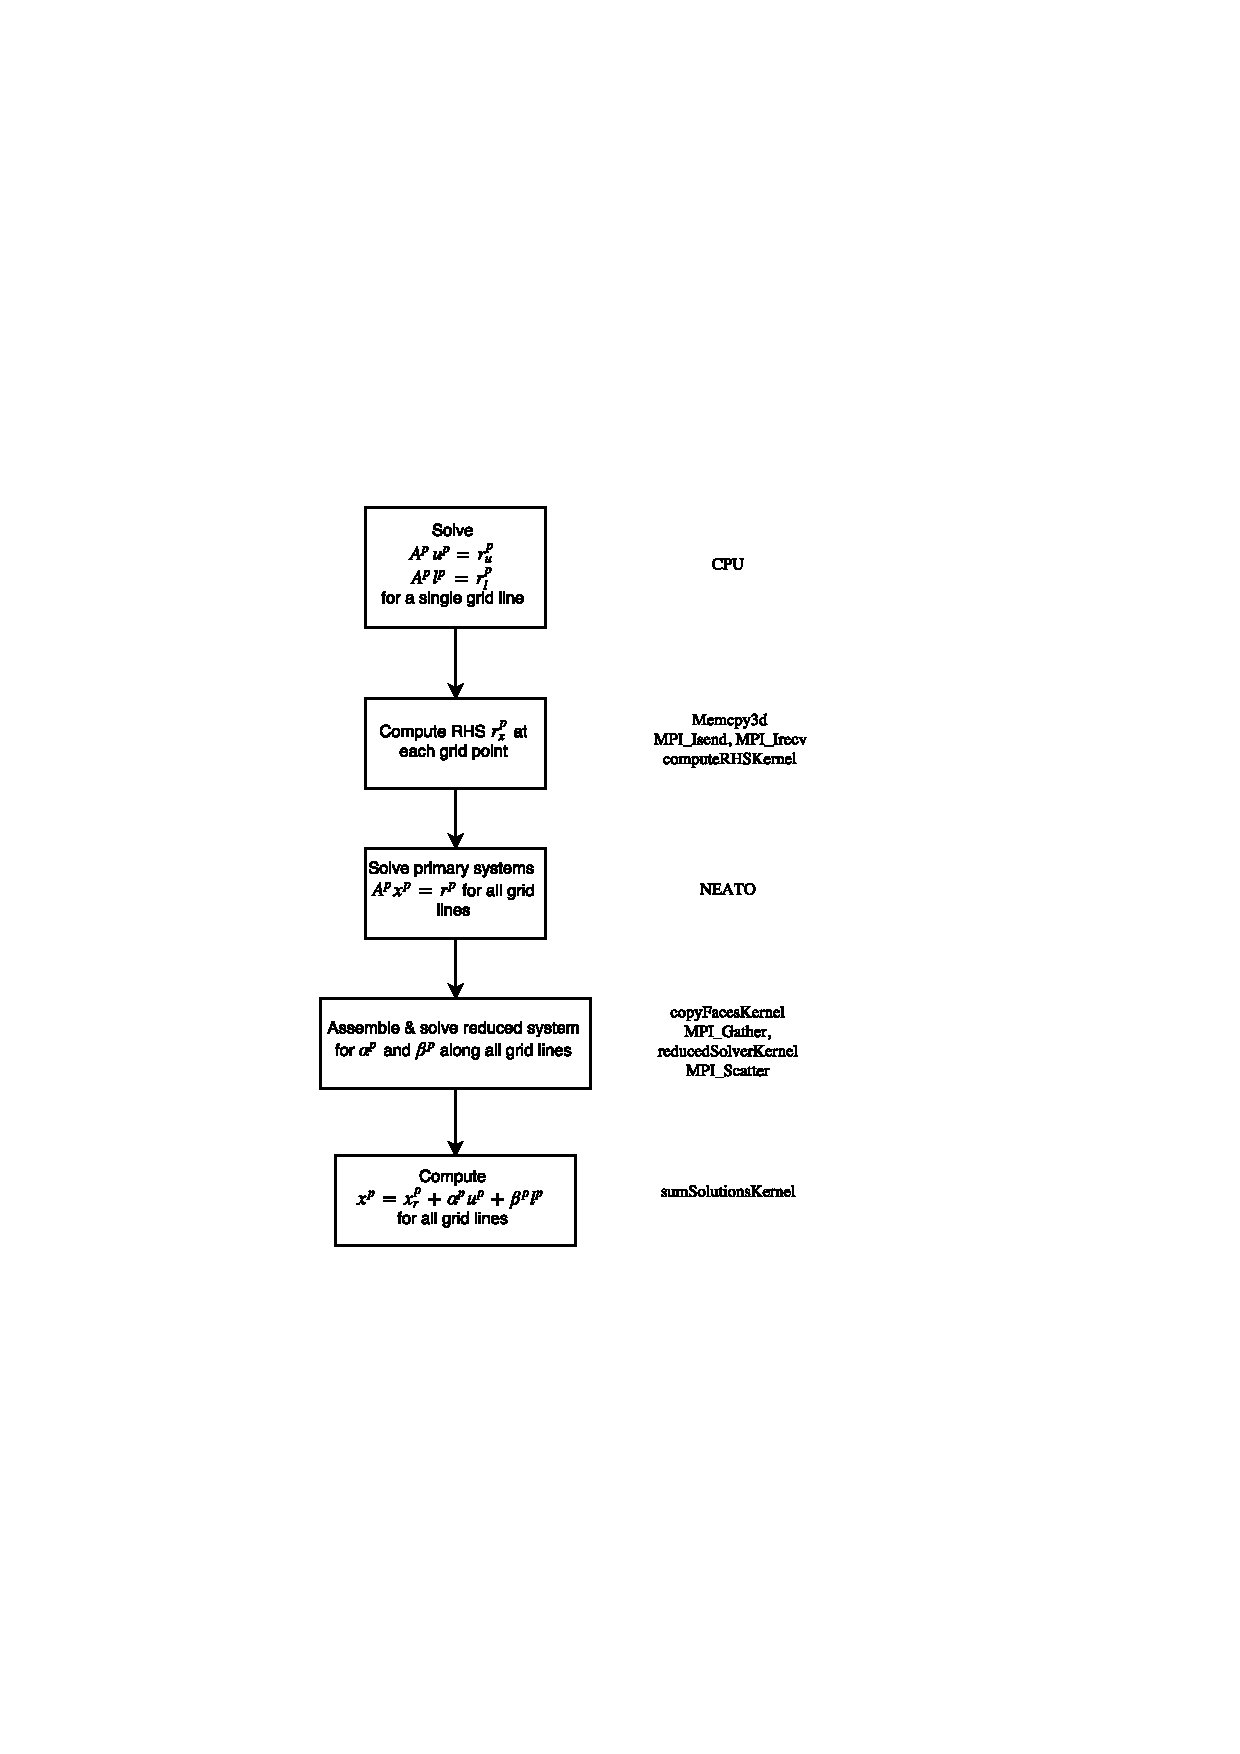
\includegraphics[trim={0 7cm 0 7cm},clip,width=500pt]{img/compact-algorithm.pdf}
\centering
\caption{Algorithm for evaluating compact finite differences on multiple GPUs,
(right: CUDA kernels and MPI calls used)}
\label{fig:compact-algorithm}
\end{center}
\end{figure}

\begin{table}[]
\centering
\caption{Purpose of kernels and MPI calls in compact finite difference application}
\label{table:compact-algorithm}
\begin{tabular}{|l|p{6cm}|}
\hline
Memcpy3d            & Copy noncontiguous boundary information
                      of the function values
                      to and from contiguous halo arrays \\ \hline
ISend, IRecv        & Perform halo swaps with i-1 and i+1 processes \\ \hline
computeRHSKernel    & Apply pointwise stencil operator to compute
                      RHS at each grid point in the subdomain,
                      using the halo values near the boundaries\\ \hline
NEATO               & Solve the primary near-Toeplitz tridiagonal systems
                      for the computed right hand sides, giving $x_r$ \\ \hline
copyFacesKernel     & Copy the left and right faces of $x_r$
                      into a single contiguous array \\ \hline
MPI\_Gather         & Gather the data required to assemble
                      the reduced system at rank 0 \\ \hline
reducedSolverKernel & Solve the reduced systems for parameters
                      $\alpha^p$ and $\beta^p$
                      for each grid line \\ \hline
MPI\_Scatter        & Scatter the parameters 
                      $\alpha^p$ and $\beta^p$
                      from rank 0 to all the processes \\ \hline
sumSolutionsKernel  & Sum the primary and secondary solutions
                      to compute the local part of the solution \\ \hline
\end{tabular}
\end{table}

\begin{figure}
\begin{center}
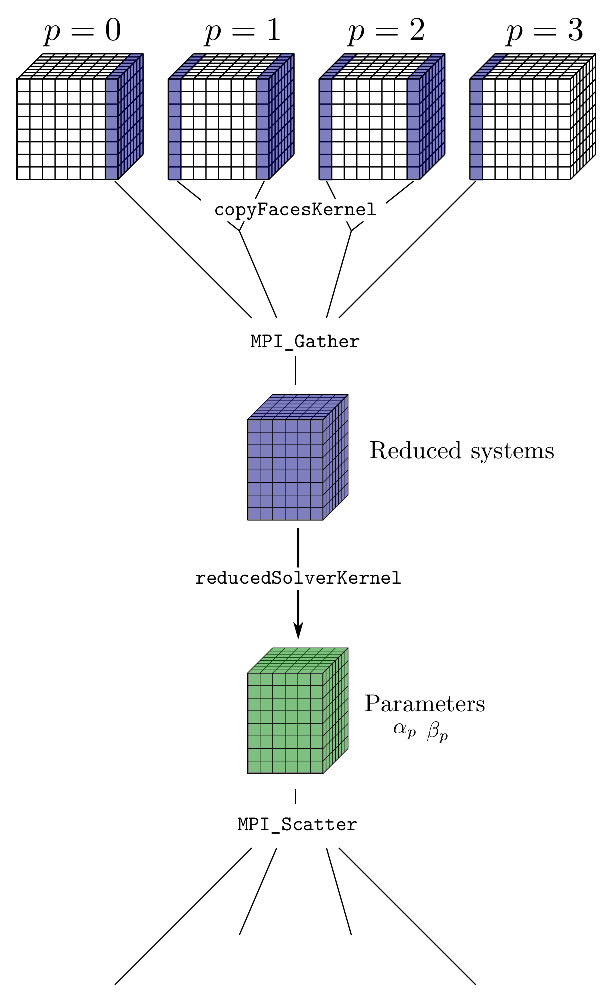
\includegraphics[width=200pt]{img/constructing-reduced-system.eps}
\caption{Construction of the reduced system and scattering of parameters.}
\label{fig:constructing-reduced-system}
\end{center}
\end{figure}
%
The secondary systems
[Eq. (\ref{eqn:secondary-system-1-expanded}) and
 Eq. (\ref{eqn:secondary-system-2-expanded})]
are solved on the CPU,
and the results are transferred to the GPU.
%
The primary system [Eq. (\ref{eqn:primary-system-expanded})] must be solved
for each of the local grid lines in a subdomain,
as the right hand sides are different at each of the local grid lines. 
The evaluation of the right hand sides are
pointwise stencil computations,
which require communication of the
function values at the boundaries of the subdomains.
This is achieved using a halo-swapping technique
with dedicated contiguous halo arrays for each subdomain,
as communication of non-contiguous MPI
data types is expensive on the GPU.
The primary system is solved for all the local grid lines
using the NEATO solver.
%
The set up and solution of the reduced system
requires global communication of the boundary information
from the solutions $\bm{u}^p$, $\bm{l}^p$ and $\bm{x_r}^p$.
The tridiagonal coefficients of the reduced system
are set up easily,
by communicating the boundary elements from
$\bm{u}^p$ and $\bm{l}^p$,
which are the same for every local grid line in each subdomain.
The right hand sides require significantly more communication,
as they are assembled from the boundary elements of $\bm{x_r}^p$,
which are different for each local grid line in each subdomain.
Thus, the boundary ``faces'' of each subdomain need to be communicated.
These faces are first copied into a contiguous array,
and these arrays are gathered at rank 0
to assemble the right-hand sides of the reduced system
(Fig. \ref{fig:constructing-reduced-system}).
This communication strategy has the effect of
producing \emph{interleaved} right hand sides
aligned along the ``slowest'' co-ordinate direction, i.e.,
the right hand side values for neighbouring grid points
are located far apart in memory.
As the reduced systems are quite small relative to the primary systems,,
we use the convenient, but rather inefficient
p-Thomas algorithm to solve the systems.
The solution of the reduced systems produces the parameters
$\alpha^p$ and $\beta^p$,
which are scattered back to the respective processes, $p$.
%
Finally, the summing of the solutions
is a pointwise operation that is easily implemented
on the GPU.
For evaluation of compact finite differences in other
coordinate directions,
a local permutation of the data is performed on the input data
(function values)
before applying the above algorithm.
and again on the output data
(derivative values).

